\documentclass[]{article}
\usepackage[a4paper, total={7in,10in}]{geometry}
\usepackage{hyperref}
\usepackage{siunitx}
\usepackage[backend=biber]{biblatex}
\addbibresource{report.bib}
\usepackage{graphicx}

%opening
\title{EP2420 - Project 1: Task 1, Task 2.1}
\author{André Silva}
\begin{document}

\maketitle

\title{\textbf{Task I}}

\begin{enumerate}

    \item
        The dataset \textit{VoD flashcrowd} provides us with $36633$ samples of $1670$ features, and $9$ different types of targets.

        In Table \ref{table:1}, the statistics for the chosen features, as well as the target \textit{DispFrames}, which represents the video frame rate, are displayed.

        \begin{table}[h!]
            \centering
            \begin{tabular}{ | c | c | c | c | c | c | c | }
                \hline
                Feature name & Mean & Std Dev & Maximum & Minimum & 25th percentile & 90th percentile \\ 
                \hline
                \textit{3\_cpu16\_.sys} & \num{3.55e+00} & \num{1.95e+00} & \num{1.50e+01} & \num{0.00e+00} & \num{0.00e+00} & \num{0.00e+00} \\
                \hline
                \textit{23\_RxPacktes} & \num{3.15e+02} & \num{4.12e+02} & \num{2.37e+03} & \num{0.00e+00} & \num{3.70e+01} & \num{4.70e+01} \\
                \hline
                \textit{3\_frmpg.s} & \num{-1.15e+01} & \num{2.07e+04} & \num{1.08e+05} & \num{-7.49e+04} & \num{-5.31e+04} & \num{-4.55e+04} \\
                \hline
                \textit{0\_cpu18\_.idle} & \num{9.97e+01} & \num{5.98e-01} & \num{1.00e+02} & \num{9.50e+01} & \num{9.70e+01} & \num{9.80e+01} \\
                \hline
                \textit{2\_cpu17\_.usr} & \num{6.03e+01} & \num{1.82e+01} & \num{9.20e+01} & \num{0.00e+00} & \num{8.00e+00} & \num{1.34e+01} \\
                \hline
                \textit{4\_cpu15\_.iowait} & \num{4.65e-03} & \num{7.21e-02} & \num{3.03e+00} & \num{0.00e+00} & \num{0.00e+00} & \num{0.00e+00} \\
                \hline
                \textit{4\_cpu5\_.sys} & \num{2.90e+01} & \num{1.08e+01} & \num{7.40e+01} & \num{0.00e+00} & \num{6.06e+00} & \num{9.18e+00} \\
                \hline
                \textit{3\_cswch.s} & \num{7.30e+04} & \num{1.79e+04} & \num{1.07e+05} & \num{7.82e+03} & \num{2.19e+04} & \num{2.65e+04} \\
                \hline
                \textit{38\_TxBytes} & \num{2.79e+06} & \num{3.18e+06} & \num{1.96e+07} & \num{0.00e+00} & \num{3.47e+05} & \num{4.63e+05} \\
                \hline
                \textit{2\_dev8.0\_avgrq.sz} & \num{2.21e+01} & \num{5.78e+01} & \num{1.02e+03} & \num{0.00e+00} & \num{0.00e+00} & \num{0.00e+00} \\
                \hline
                \textit{DispFrames} & \num{2.20e+01} & \num{4.32e+00} & \num{2.50e+01} & \num{0.00e+00} & \num{3.00e+00} & \num{8.00e+00} \\
                \hline
            \end{tabular}
            \caption{Statistics for chosen features and target}
            \label{table:1}
        \end{table}

        The following list gives a short description of these features. This information was retrieved from linux manual pages for the command \texttt{sar}~\cite{sar}.

        \begin{itemize}
            \item \textit{3\_cpu16.sys} - Percentage of CPU utilization that occurred while executing at the system level (kernel).
            \item \textit{23\_RxPackets} - Total number of packets received per second.
            \item \textit{3\_frmpg.s} - Number of memory pages freed by the system per second.
            \item \textit{0\_cpu18\_.idle} - Percentage of time that the CPU or CPUs were idle and the system did not have an outstanding disk I/O request.
            \item \textit{2\_cpu17\_.usr} - Percentage of CPU utilization that occurred while executing at the user level (application).
            \item \textit{4\_cpu15\_.iowait} - Percentage of time that the CPU was idle during which the system had an outstanding disk I/O request.
            \item \textit{4\_cpu5\_.sys} - Percentage of CPU utilization that occurred while executing at the system level (kernel).
            \item \textit{3\_cswch.s} - Total number of context switches per second.
            \item \textit{38\_TxBytes} - Total number of bytes transmitted per second.
            \item \textit{2\_dev8.0\_avgrq.sz} - The average size (in sectors) of the requests that were issued to the device.
        \end{itemize}
\end{enumerate}

\pagebreak

\title{\textbf{Task II - 2.1}}

\begin{enumerate}
    \item [4.]
        Table \ref{table:2} provides the calculated \textit{Normalized Mean Absolute Error} (\textsc{NMAE}) for each of the regressors. 
        The parameters utilized for the random forest regression and the neural network regression are the default parameters of, respectively, \texttt{RandomForestRegressor}~\cite{RFR} and \texttt{MLPRegressor}~\cite{MLPR}, unless specified in the table.
        \begin{table}[h!]
            \centering
            \begin{tabular}{ | c | c | }
                \hline
                Regressor & \textsc{NMAE} \\ 
                \hline
                \texttt{LinearRegression} & \num{0.318} \\ 
                \hline
                \texttt{RandomForestRegressor(n\_estimators=10)} & \num{0.087}\\ 
                \hline
                \texttt{MLPRegressor(max\_iter=1000, activation='logistic', hidden\_layers=(10,10))} & \num{0.144}\\ 
                \hline
            \end{tabular}
            \caption{\textit{Normalized Mean Absolute Error} for each regressor tested}
            \label{table:2}
        \end{table}

        \begin{figure}[h!]
        \centering
        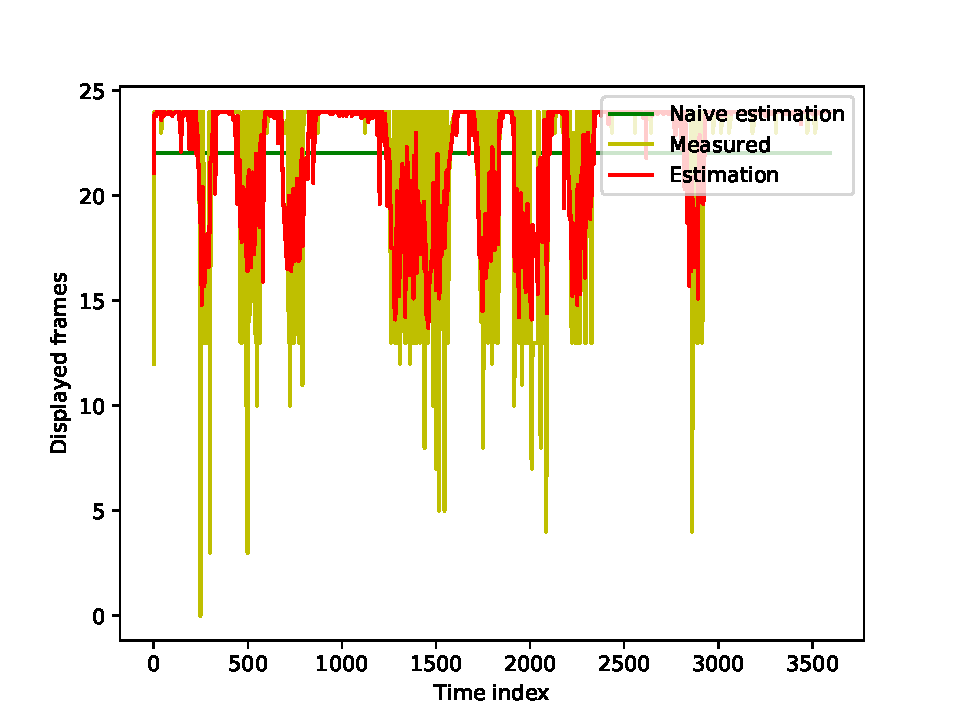
\includegraphics[width=\textwidth,height=\textheight,keepaspectratio]{../result/project1/rfr.pdf}
        \caption{Time series plot for \textit{VoD flashcrowd} using \texttt{RnadomForestRegressor}}
        \end{figure}

        \begin{figure}
        \centering
        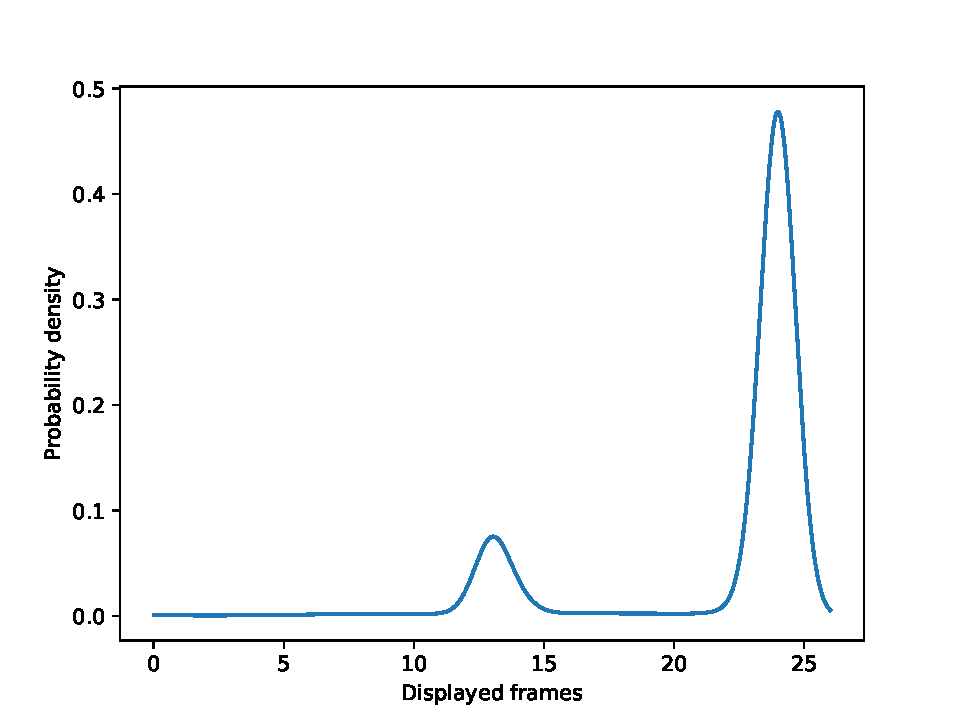
\includegraphics[width=\textwidth,height=0.25\textheight,keepaspectratio]{../result/project1/frames_density.pdf}
        \caption{Density plot of the target values in the test set}
        \end{figure}

        \begin{figure}
        \centering
        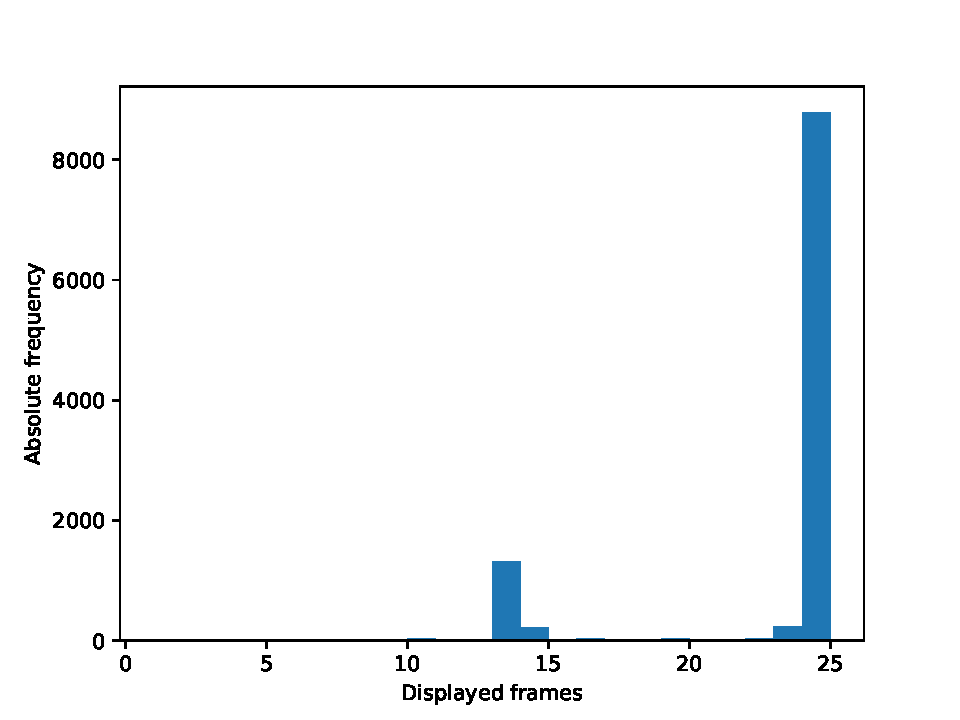
\includegraphics[width=\textwidth,height=0.25\textheight,keepaspectratio]{../result/project1/frames_hist.pdf}
        \caption{Histogram of the target values in the test set}
        \end{figure}

        \begin{figure}
        \centering
        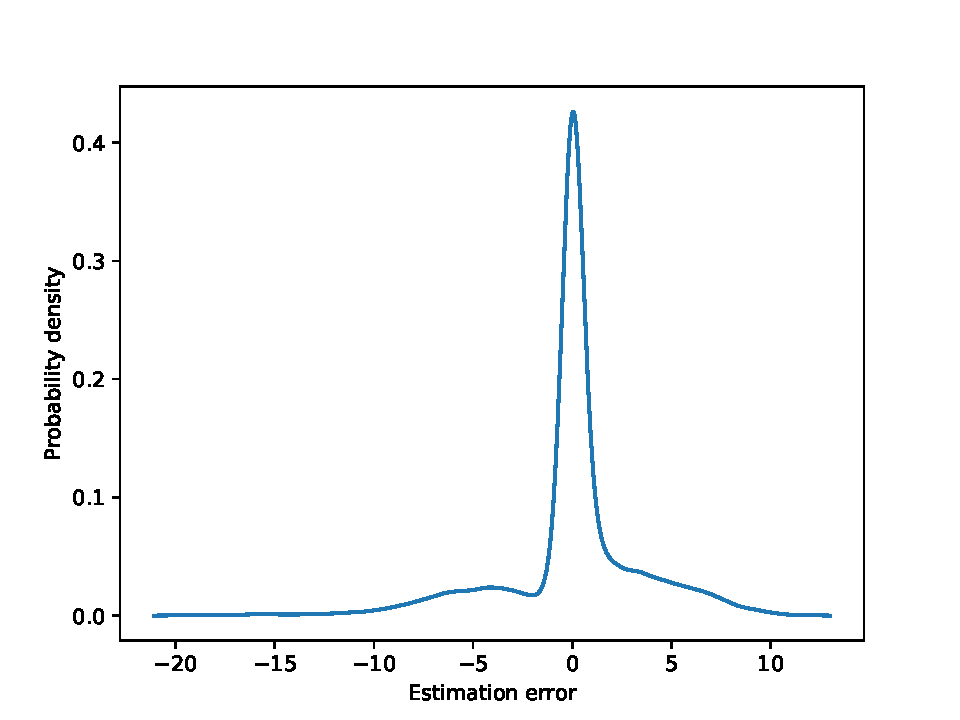
\includegraphics[width=\textwidth,height=0.25\textheight,keepaspectratio]{../result/project1/error_density.pdf}
        \caption{Density plot of the estimation errors $y_i - \hat{y}_i$ in the test set}
        \end{figure}

    \clearpage

    \item [9.]
        Of the three regression techniques utilized, linear regression was the least expensive in computational power, but also the one which provided the worst accuracy. 

        Neural network regression was more expensive when compared to random forest regression, but provided worse accuracy.

        Random forest regression was better both in terms of accuracy and cost-performance trade-off when compared to the other two models.

\end{enumerate}

\printbibliography

\end{document}
